\documentclass{report}
\usepackage[margin=1in]{geometry}
\usepackage[T1]{fontenc} % Fontes T1
\usepackage[utf8]{inputenc} % Input UTF8
\usepackage{csquotes}
\usepackage[portuguese]{babel} %Usar língua portuguesa
\usepackage{blindtext} % Gerar texto automaticamente
\usepackage[printonlyused]{acronym}
\usepackage{hyperref} % para autoref
\usepackage{graphicx}
\usepackage{subcaption}
\usepackage{float}
\usepackage{listings}
\usepackage{color}

\definecolor{dkgreen}{rgb}{0,0.6,0}
\definecolor{gray}{rgb}{0.5,0.5,0.5}
\definecolor{mauve}{rgb}{0.58,0,0.82}

\lstset{frame=tb,
  language=Python,
  aboveskip=3mm,
  belowskip=3mm,
  showstringspaces=false,
  columns=flexible,
  basicstyle={\small\ttfamily},
  numbers=none,
  numberstyle=\tiny\color{gray},
  keywordstyle=\color{blue},
  commentstyle=\color{dkgreen},
  stringstyle=\color{mauve},
  breaklines=true,
  breakatwhitespace=true,
  tabsize=3
}

\graphicspath{{./imagens/}}

\begin{document}
	\begin{titlepage}
    	\begin{center}
    		
\includegraphics[width=0.6\textwidth]{logo-isec}
    		
    		\vspace*{\fill}
    		
    		\Huge
    		\textbf{Relatório Preliminar - Balanceamento de carga em Servidores Web com HAProxy e Keepalived}
    		
    		\huge
    		Disponibilidade e Desempenho
    		
    		\vspace{0.5cm}
    		\LARGE
    		2021 - 2022
    		
    		\vspace{1.5cm}
    		
    		\textbf{Bruno Teixeira}\\
                a2019100036@isec.pt
    		
    		\vfill
    		\vspace*{\fill}
    		
    		\normalsize
    		Licenciatura de Engenharia Informática \\
    		22 de dezembro de 2021
    	\end{center}
    \end{titlepage}

\pagenumbering{roman}


\tableofcontents
% \listoftables     % descomentar se necessário
\listoffigures    % descomentar se necessário


%%%%%%%%%%%%%%%%%%%%%%%%%%%%%%%
\clearpage
\pagenumbering{arabic}

%%%%%%%%%%%%%%%%%%%%%%%%%%%%%%%%

\chapter{Introdução}\label{chap.introducao}
\paragraph{}
Este trabalho tem como objetivo estudar o balanceamento de carga e o \emph{failover} em servidores \emph{web} com o HAProxy e o KeepAlived. \\
O principal foco é, criar alguns cenários com possíveis falhas, analizar esses cenários, descobrir os pontos fracos e tentar sempre minimizar o \emph{down-time}.
\paragraph{}
Para alcançar este objetivo foram então criadas algumas experiências de modo a perceber como é possível criar uma infraestrutura segura e com um \emph{down-time} reduzido ou até mesmo nulo aplicando ao mesmo tempo o conceito de balanceamento de carga.

\chapter{Desenvolvimento}\label{Desensolvimento}

\section{Descrição das tecnologias usadas}

\section{Flask, MariaDB e Galera Cluster}
\paragraph{}
O Flask é um \emph{micro-framework} do \emph{Python} destinado principalmente para pequenas aplicações com requisitos mais simples. O mesmo funciona bastante bem com bases de dados tendo sido este o escolhido para o desenvolvimento da aplicação \emph{web} para este trabalho.\\
Para que a aplicação fosse \emph{stateful} foi então usada uma base de dados em MariaDB, uma vez que a mesma tem uma comunidade enorme na Internet, tornando-a bastante simples de ser utilizada.

\paragraph{}
O \emph{Galera Cluster} é um \emph{cluster} virtual para MariaDB que permite a replicação entre diferentes bases de dados, mantendo assim uma disponibilidade e desempenho alto uma vez que existe mais do que uma base de dados para responder a diferentes \emph{querys} dos clientes, sendo que todas as mudanças feitas numa base de dados são replicadas para a outra.


\section{HAProxy}
\paragraph{}
O HAProxy é um serviço Linux que garante o balanceamento de carga para HTTP e TCP. Na prática, o mesmo recebe as conexões dos utilizadores e atua como \emph{proxy}, criando um canal de comunicação entre o utilizador e um dos \emph{webservers}.

\paragraph{}
O HAProxy funciona em dois modos diferentes, HTTP ou TCP.

\begin{itemize}
  \item Quando opera em TCP dizemos que é um \emph{Proxy} de camada 4 (OSI)
        \begin{itemize}
          \item Quando o HAProxy opera neste modo, o mesmo apenas tem acesso a qual IP e Porto o cliente está a tentar aceder, não conseguindo assim ver a informação trocada entre de ambas as partes.
        \end{itemize}
  \item Quando opera em HTTP dizemos que é um \emph{Proxy} de camada 7 (OSI)
    \begin{itemize}
      \item Quando o HAProxy opera neste modo, o mesmo tem acesso a toda a informação, logo estamos a confiar no mesmo para ter acesso a esses dados, dados que transitam de um lado para o outro.
        \end{itemize}
\end{itemize}


\section{KeepAlived}
\paragraph{}
O objetivo principal do KeepAlived é fornecer instalações simples para existir balanceamento de carga e alta disponibilidade (a alta disponibilidade é alcançada pelo protocolo VRRP) para sistemas baseados em Linux. O Keepalived agrega então um conjunto de servidores de balanceamento de carga (HAProxy), e consoante a saúde dos mesmos, ele toma decisões sobre pelo qual deverá passar a operacionalização.


\section{Ambiente para as experiências}
\paragraph{}
Para serem feitas algumas experiências foi criado um ambiente com várias máquinas virtuais, estando estas agregadas a um virtualizador ESXi, ou seja, todas as máquinas estão na mesma LAN.

\begin{itemize}
  \item \textbf{webserver01} - 192.168.1.180
  \item \textbf{webserver02} - 192.168.1.181

  \item \textbf{mariadb01} - 192.168.1.182
  \item \textbf{mariadb02} - 192.168.1.186
    
  \item \textbf{haproxy01} - 192.168.1.183
  \item \textbf{haproxy02} - 192.168.1.184
    
  \item \textbf{haproxy03} - 192.168.1.185
  \item \textbf{haproxy04} - 192.168.1.187
\end{itemize}

\subsection{Aplicação Web}
\paragraph{}
Como descrito anteriormente, foi criada uma aplicação em Flask. Esta aplicação funciona como uma espécie de lista de compras em que o utilizador depois de fazer o \emph{login}, consegue adicionar e eliminar produtos do seu cesto.

\begin{figure}[H]
\center
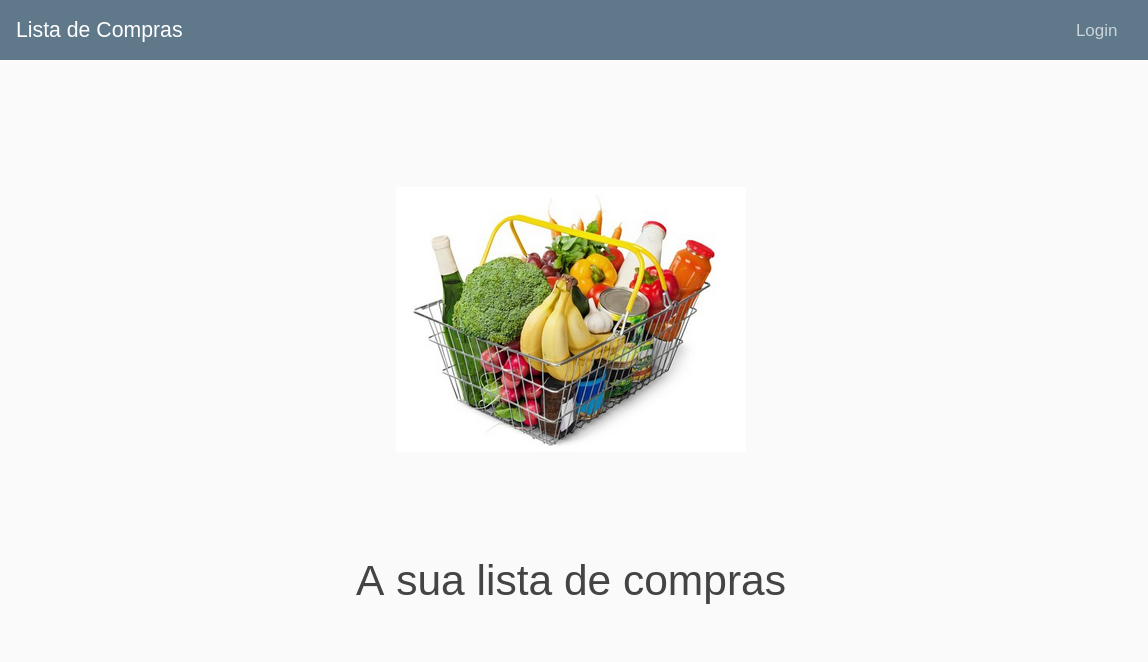
\includegraphics[width=12cm]{imagens/aplicacao_web/index.png}
\caption{Index - Aplicação Web} 
\label{fig.nav}
\end{figure}


\begin{figure}[H]
\center
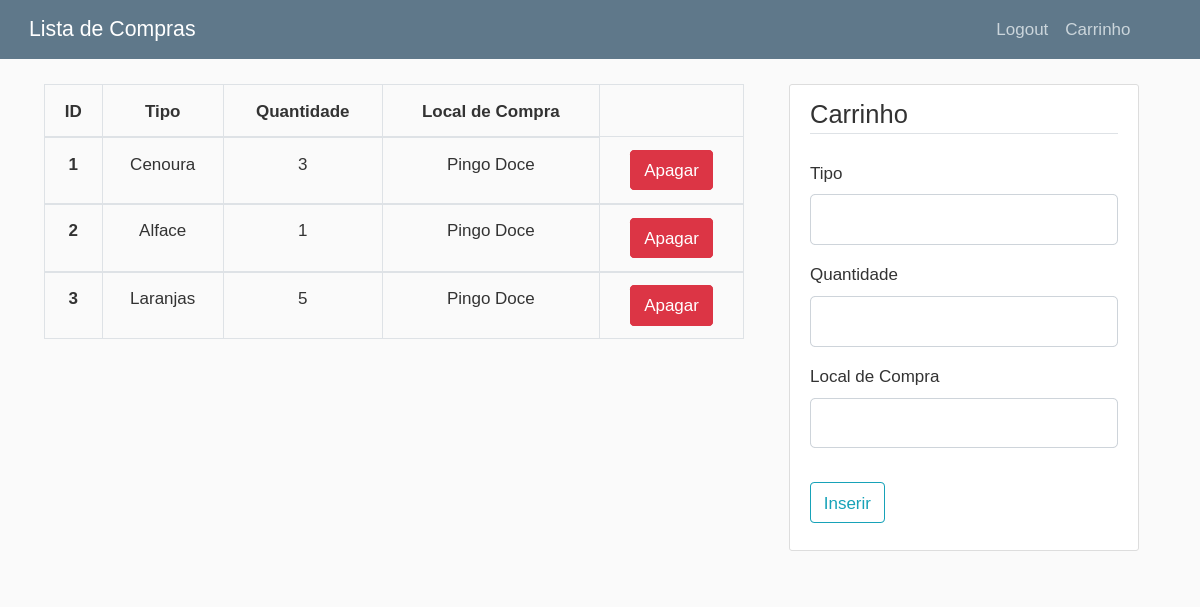
\includegraphics[width=12cm]{imagens/aplicacao_web/carrinho.png}
\caption{Carrinho - Aplicação Web}
\label{fig.nav}
\end{figure}

\subsection{Configuração do HAProxy}
\paragraph{}
No ficheiro de configuração do HAProxy (localizado em \textbf{\emph{/etc/haproxy/haproxy.cfg}}) existem 5 secções, sendo que estas definem como é que o servidor se comporta, quais são as definições por omissão, e como é que o cliente faz pedidos e recebe respostas.
\begin{itemize}
  \item \textbf{global}
    \begin{itemize}
      \item Nesta primeira secção estão definidas as medidas em que o processo vai operar, sendo estas medidas de um nível mais baixo, ou seja, relacionadas com o sistema operativo.
    \end{itemize}
          
  \item \textbf{defaults}
    \begin{itemize}
      \item Esta secção não é obrigatória, no entanto permite reduzir a duplicação de comandos, uma vez que as configurações feitas aqui são aplicadas na secção \textbf{\emph{frontend}} e \textbf{\emph{backend}}.
    \end{itemize}
      
  \item \textbf{listen}
    \begin{itemize}
      \item Aqui podemos combinar o \textbf{frontend} e \textbf{backend} ao mesmo tempo. Isto é útil, pois é aqui feito o redirecionamento para o \textbf{\emph{endpoint}} de estatisticas.
     \end{itemize}
      
   \item \textbf{frontend}
     \begin{itemize}
       \item Nesta secção definimos como é que os pedidos dos utilizadores irão ser encaminhados para o \textbf{backend}.
     \end{itemize}

       
   \item \textbf{backend}
     \begin{itemize}
       \item Aqui definimos os \textbf{\emph{webservers}} que vão operar na infraestrutura, definindo tambem o algoritmo de \textbf{\emph{load balancing}} a ser utilizado
     \end{itemize}
\end{itemize}


\begin{figure}[H]
\center
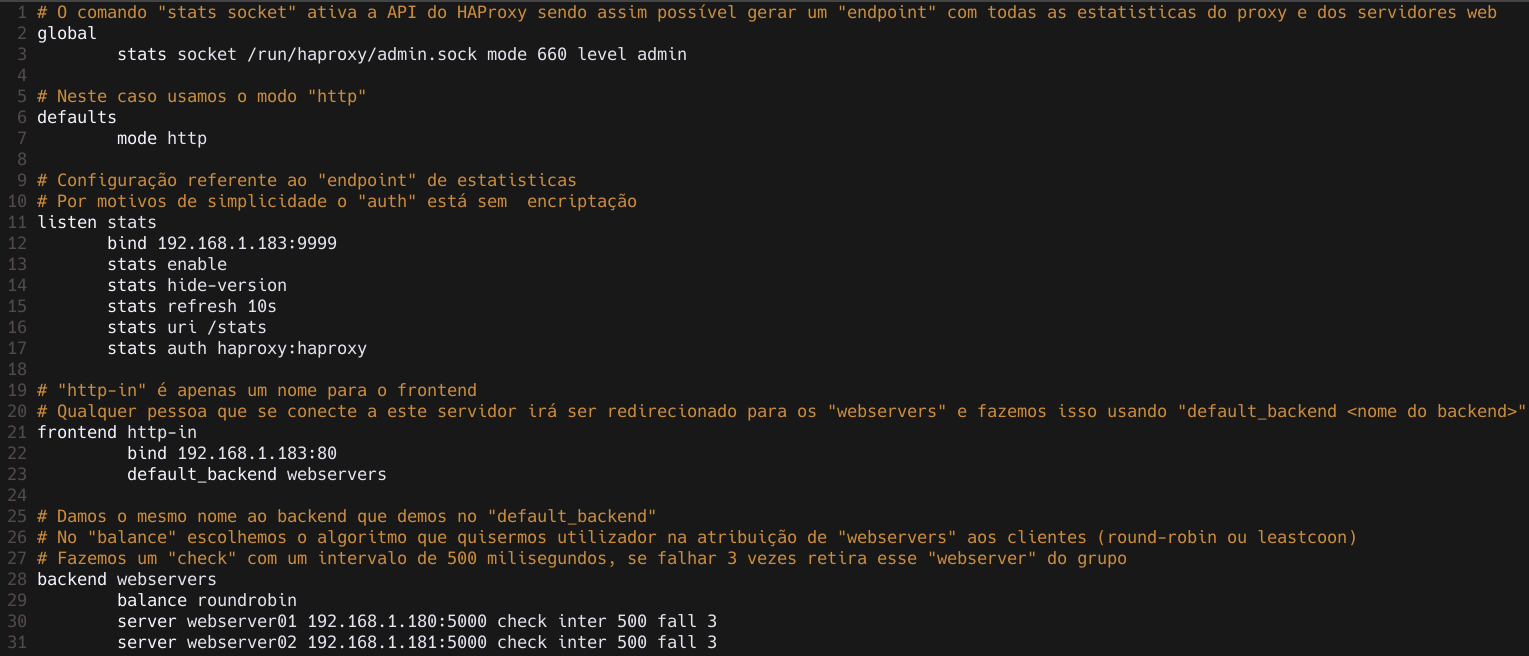
\includegraphics[width=16cm]{imagens/haproxy_config.png}
\caption{Configuração - HAProxy}
\label{fig.nav}
\end{figure}

Conforme foi configurado o HAProxy, ao acedermos a \textbf{\emph{http://192.168.1.183:9999/stats}} conseguimos visualizar uma página \emph{web} com várias estatísticas sobre os \emph{webservers}. 

\begin{figure}[H]
\center
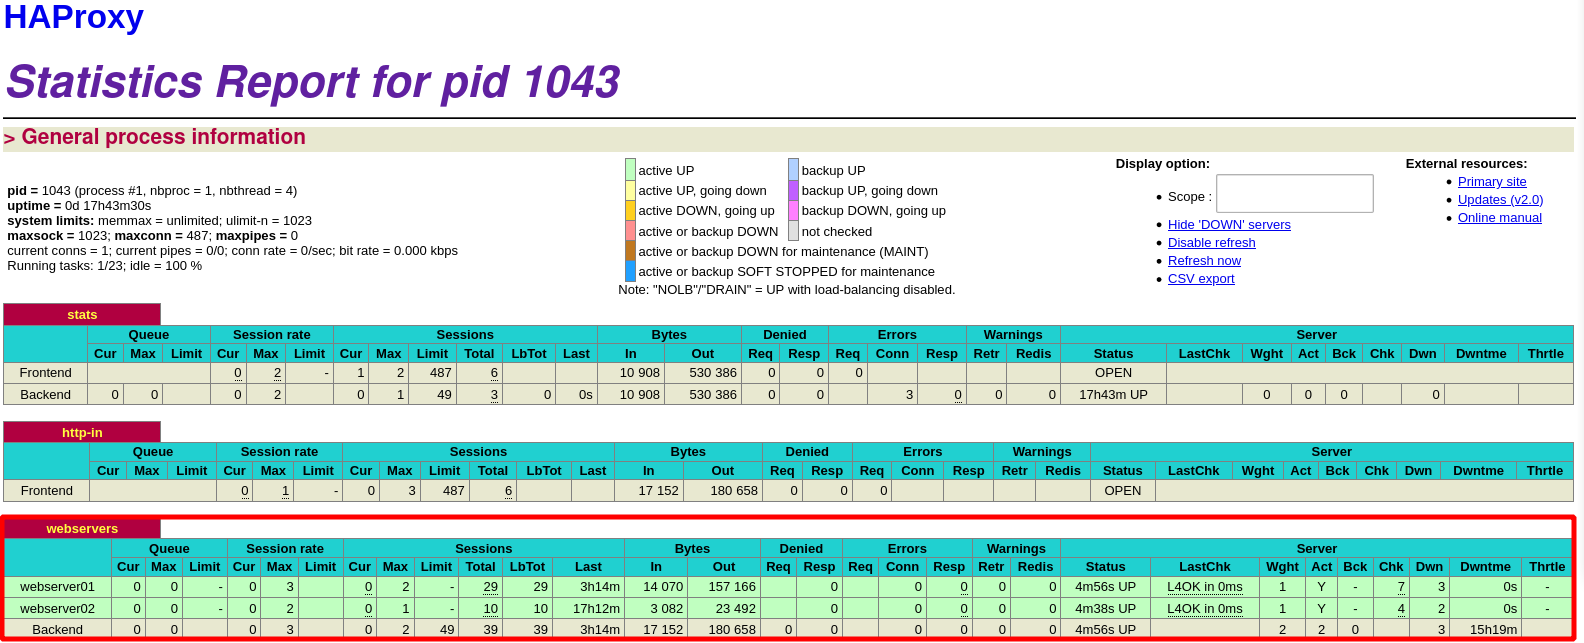
\includegraphics[width=17cm]{imagens/haproxy_stats.png}
\caption{Estatísticas - HAProxy}
\label{fig.nav}
\end{figure}


\subsection{Configuração do KeepAlived}
\paragraph{}
No ficheiro de configuração do Keepalived (localizado em \textbf{\emph{/etc/keepalived/keepalived.conf}}), foi criado um \textbf{vrrp\_script} com o intuito de verificar, com um intervalo de 2 em 2 milisegundos, se o haproxy está a funcionar corretamente. Se o mesmo não estiver a funcionar, o peso dele diminui em 10 reduzindo assim a sua prioridade tornando o BACKUP num MASTER.\\
Depois disto, foi criado um \textbf{vrrp\_instance} que define uma instância individual do protocolo VRRP com alguns atributos.

\begin{figure}[H]
\center
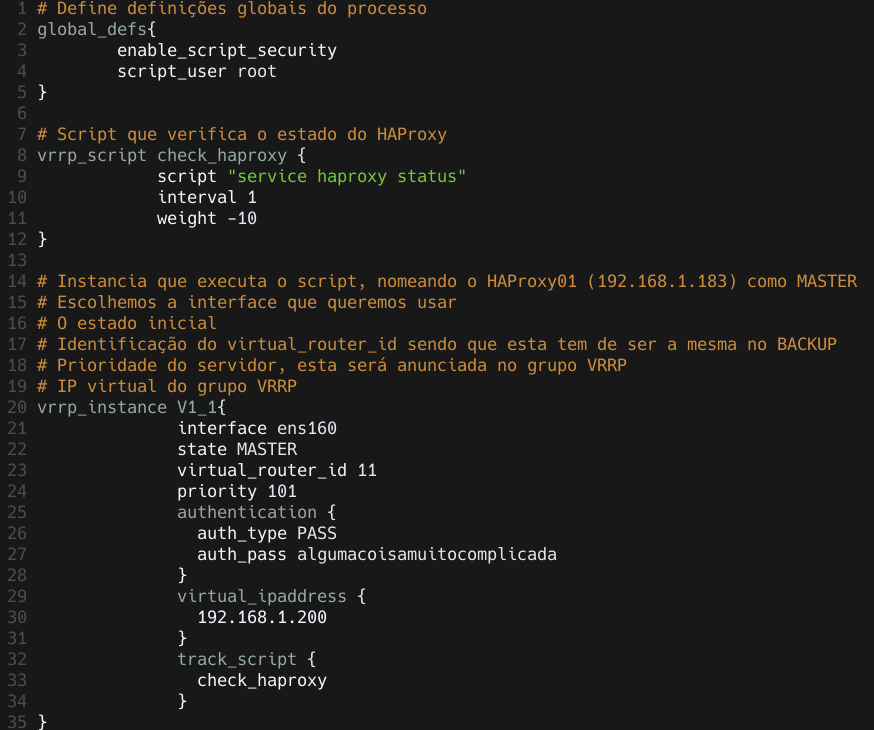
\includegraphics[width=11cm]{imagens/keepalived_config.png}
\caption{Configuração - Keepalived}
\label{fig.nav}
\end{figure}

O mesmo foi feito para o segundo servidor de HAProxy, no entanto foi alterada a prioridade e o estado para definir que este seria o BACKUP.\\

Foi tambem necessário alterar o Ip, para onde faziamos \textbf{\emph{bind}} inicialmente (\textbf{Ip do servidor HAProxy}),  para o novo IP virtual (\textbf{192.168.1.200}) na secção de \textbf{\emph{frontend}} do ficheiro de configuração do HAProxy.

Por fim foi preciso colocar \textbf{\emph{net.ipv4.ip\_nonlocal\_bind=1}} no ficheiro \textbf{\emph{/etc/sysctl.conf}} uma vez que no segundo servidor de HAProxy o IP virtual ainda não está ativo (só fica ativo quando esse for o MASTER), logo não é possível iniciar o \emph{bind}.

\paragraph{}
Esta configuração do KeepAlived apenas foi feita a partir da segunda experiência, uma vez que na primeira ainda não é usado o mesmo para mostrar os riscos que isso tem.

\section{Experiências}

\subsection{Experiência 01}
\paragraph{}
Nesta experiência foi usado um servidor de balanceamento de carga (HAProxy), dois \emph{webservers} e uma base de dados externa (MariaDB). Foi feita uma captura no HAProxy para perceber o que acontecia quando o utilizador fazia um pedido ao mesmo.

\begin{figure}[H]
\center
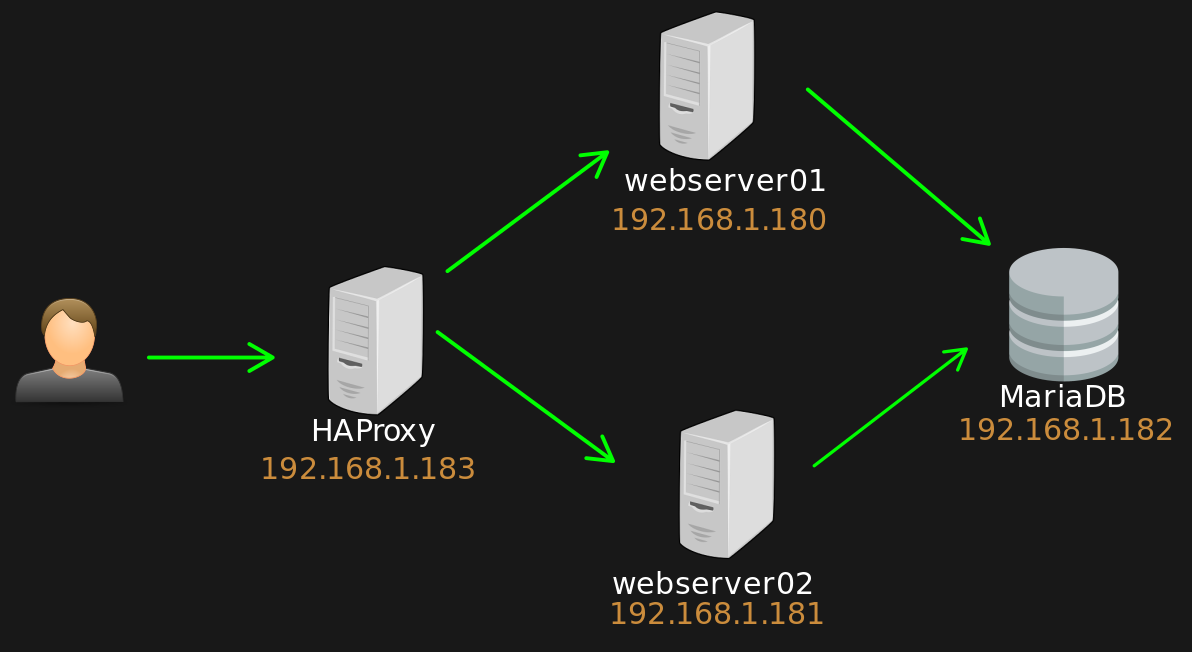
\includegraphics[width=12cm]{imagens/experiencias/01_1.png}
\caption{Esquema - Experiência 01}
\label{fig.nav}
\end{figure}


\subsubsection{Resultado}
Conseguiu-se perceber que o cliente (\textbf{192.168.1.123}) envia um \emph{HTTP GET Request} diretamente ao servidor HAProxy (\textbf{192.168.1.183}).
De seguida, o servidor HAProxy faz um \emph{HTTP GET Request} ao \emph{webserver} disponível, que neste caso foi o \emph{webserver01} (\textbf{192.168.1.180}).
O \emph{webserver01} responde com o \emph{HTTP status code 200}, mostrando que a comunicação ocorreu sem falhas, sendo feito depois um redirecionamento do HAProxy para o cliente.
Imediatamente a seguir foi feito outro pedido pelo mesmo cliente, no entanto consegue-se perceber que, como está a ser usar o algoritmo \textbf{round-robin}, quem respondeu foi o \emph{webserver02}.

\begin{figure}[H]
\center
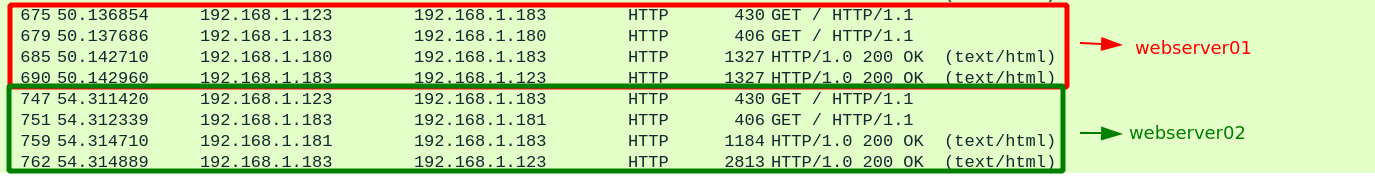
\includegraphics[width=16cm]{imagens/experiencias/01_wireshark.png}
\caption{Wireshark - Experiência 01}
\label{fig.nav}
\end{figure}

\subsubsection{Problemas encontrados na Experiência 01}
\paragraph{}
É percetivel que a experiência feita anteriormente tem alguns problemas, como a existência de dois SPOFs (\textbf{Single Point of Failure}).
\begin{itemize}
  \item Existe um SPOF no HAProxy.
  \item Existe um SPOF na Base de Dados.
\end{itemize}
Ou seja, caso o servidor de HAProxy ou a base de dados deixe de operar, o cliente deixa de ter comunicação com os \emph{webservers}. Sabendo isto continuou-se com mais algumas experiências de modo a resolver estes problemas.

\begin{figure}[H]
\center
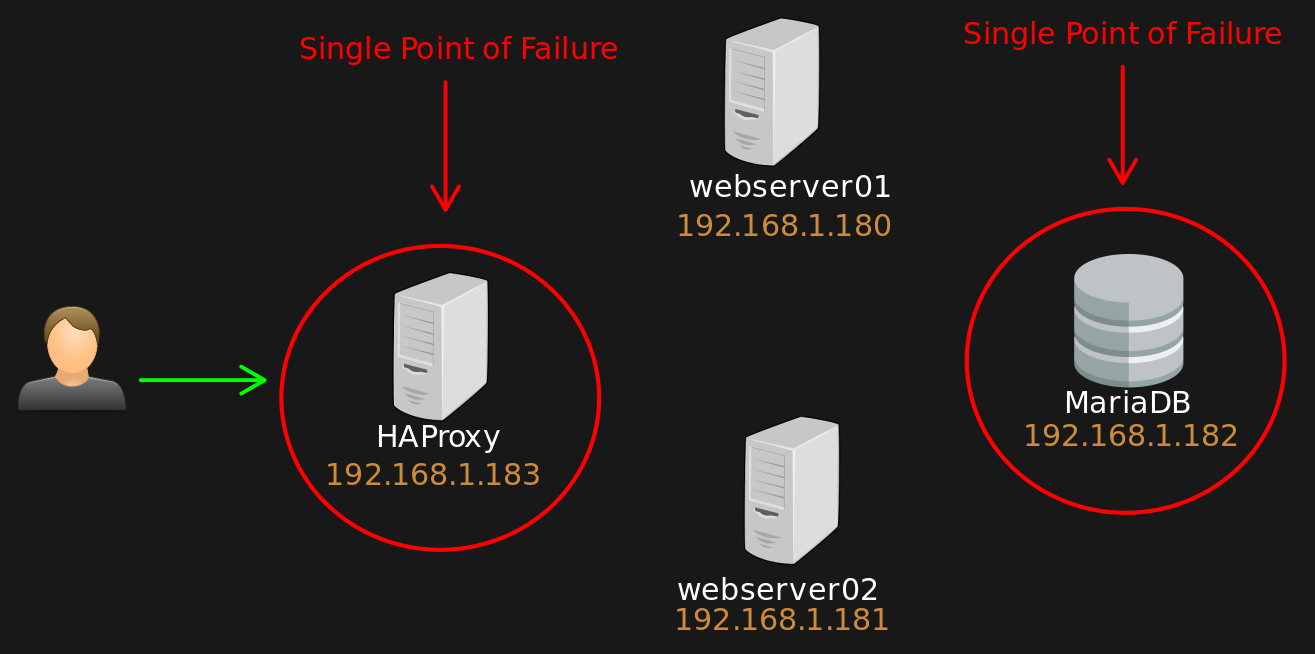
\includegraphics[width=12cm]{imagens/experiencias/01_spof.png}
\caption{Single Point of Failure - Experiência 01}
\label{fig.nav}
\end{figure}


\subsection{Experiência 02}
Nesta segunda experiência apenas foi acrescentado mais um servidor de balanceamento de carga e o serviço de \textbf{KeepAlived} em ambos os servidores de HAProxy.\\
O objetivo da mesma era entender como seria feito o \emph{fail-over} do \textbf{KeepAlived} e o que sucedia depois de um servidor \emph{MASTER} tornar-se \emph{BACKUP} e vice-versa.

\begin{figure}[H]
\center
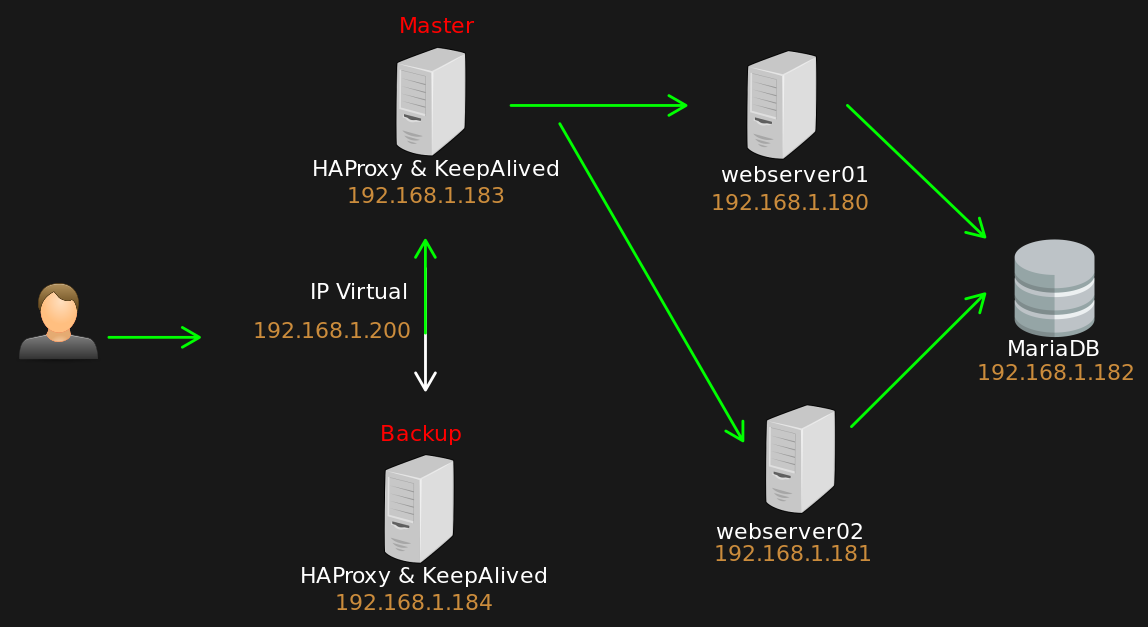
\includegraphics[width=12cm]{imagens/experiencias/02_01.png}
\caption{Esquema inicial - Experiência 02}
\label{fig.nav}
\end{figure}

\begin{figure}[H]
\center
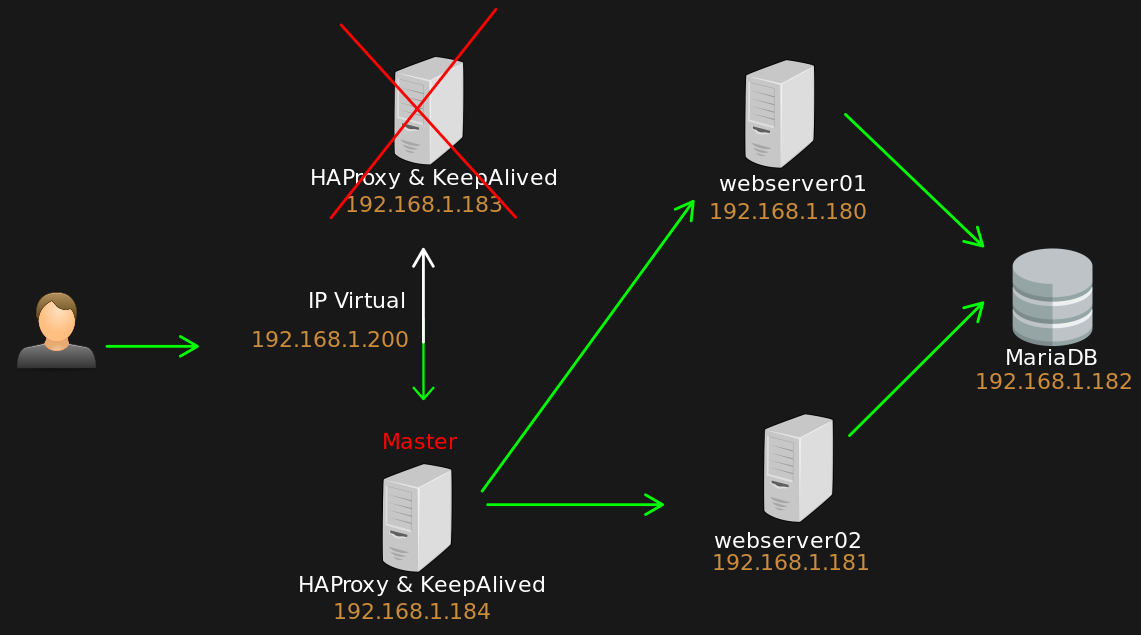
\includegraphics[width=12cm]{imagens/experiencias/02_02.png}
\caption{Esquema com \emph{fail-over} - Experiência 02}
\label{fig.nav}
\end{figure}


\subsubsection{Resultado}
Foram feitas várias capturas, tanto no \textbf{HAProxy01(MASTER)} como no \textbf{HAProxy02(BACKUP)} usando o \emph{wireshark}.\\
Com a captura no \textbf{HAProxy01(192.168.1.183)} percebe-se que o mesmo emite, de segundo em segundo, um \emph{announcement} dizendo a sua prioridade, que neste caso é 101. Isto acontece porque no protocolo VRRP apenas o \emph{MASTER} emite mensagens estando os outros \emph{BACKUPs} à escuta desse aviso.

\begin{figure}[H]
\center
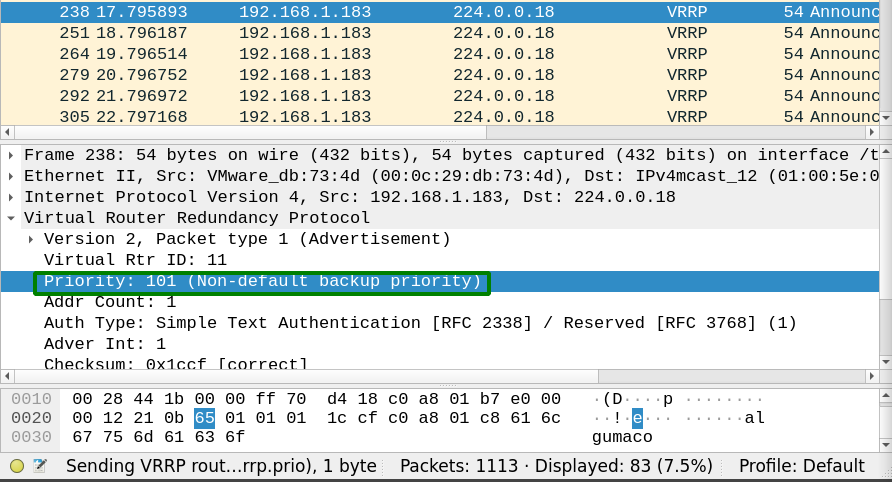
\includegraphics[width=12cm]{imagens/experiencias/02_wireshark.png}
\caption{Wireshark no 192.168.1.183 - Experiência 02}
\label{fig.nav}
\end{figure}

\begin{figure}[H]
\center
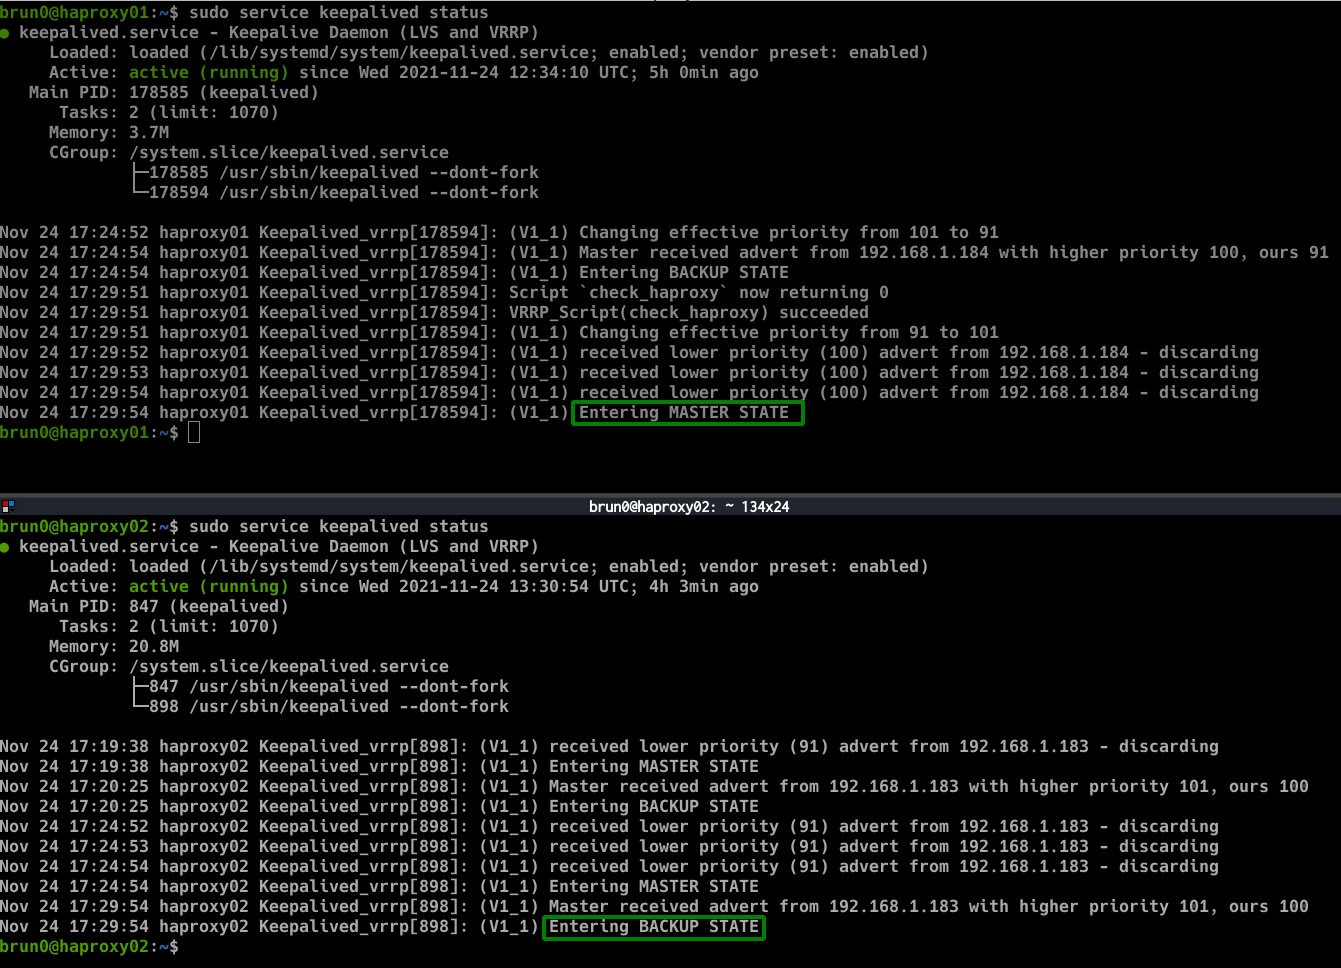
\includegraphics[width=14cm]{imagens/experiencias/02_terminal.png}
\caption{Estado inicial do KeepAlived em ambos os servidores - Experiência 02}
\label{fig.nav}
\end{figure}


\paragraph{}
Depois de desligar o serviço HAProxy do \textbf{HAProxy01(192.168.1.183)}, o mesmo fica com uma prioridade de 91 passando assim para o estado de \emph{BACKUP} ao mesmo tempo que o \textbf{HAProxy02(192.168.1.184)} passa para o estado de \emph{MASTER} uma vez que a sua prioridade é superior (100).

\begin{figure}[H]
\center
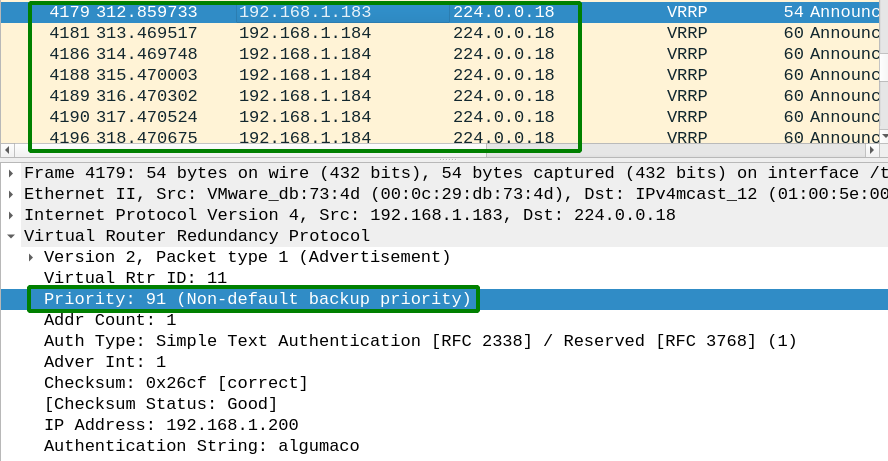
\includegraphics[width=12cm]{imagens/experiencias/02_wireshark_haproxy_desligado.png}
\caption{Wireshark no 192.168.1.183 com o HAProxy desligado - Experiência 02}
\label{fig.nav}
\end{figure}

\begin{figure}[H]
\center
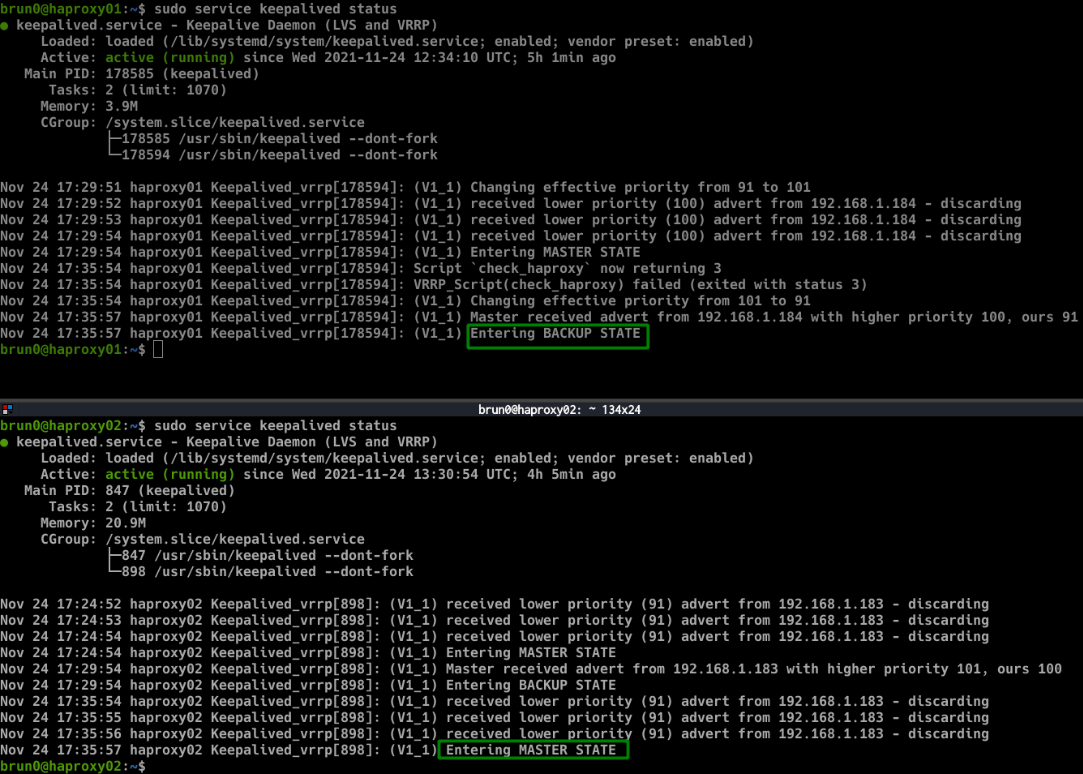
\includegraphics[width=14cm]{imagens/experiencias/02_terminal_haproxy_desligado.png}
\caption{Estado atual do KeepAlived em ambos os servidores - Experiência 02}
\label{fig.nav}
\end{figure}

\paragraph{}
Para terminar, voltou-se a ativar o serviço haproxy no \textbf{HAProxy01(192.168.1.183)} tornando-se assim novamente \emph{MASTER} uma vez que a preempção está ativa por omissão fazendo com que a sua prioridade volte a ser 101 como estava definida inicialmente.

\begin{figure}[H]
\center
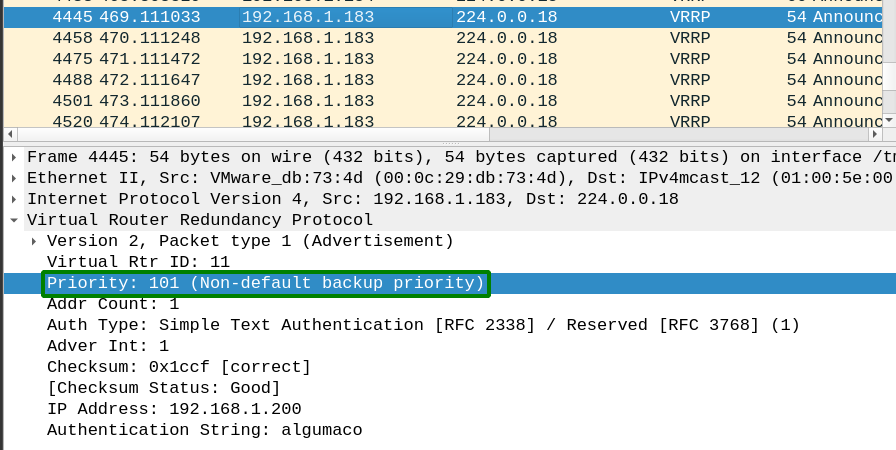
\includegraphics[width=12cm]{imagens/experiencias/02_wireshark_haproxy_retomado.png}
\caption{Wireshark no 192.168.1.183 com o HAProxy retomado - Experiência 02}
\label{fig.nav}
\end{figure}

\begin{figure}[H]
\center
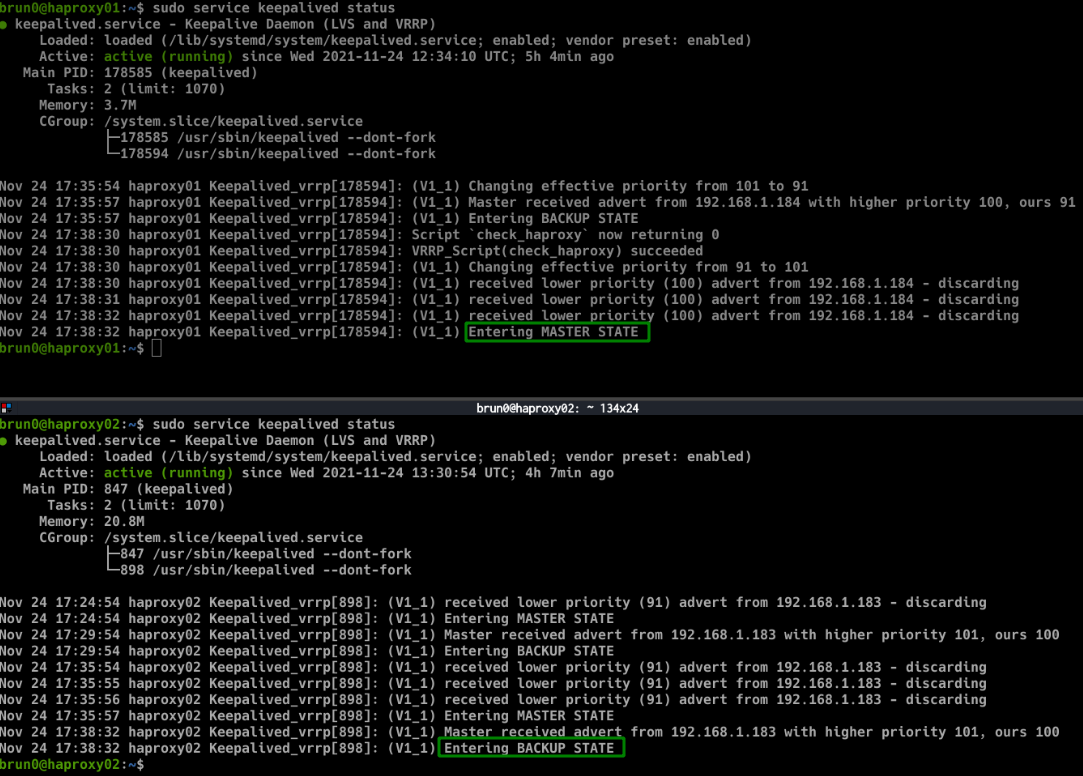
\includegraphics[width=14cm]{imagens/experiencias/02_terminal_haproxy_retomado.png}
\caption{Estado final do KeepAlived - Experiência 02}
\label{fig.nav}
\end{figure}

\subsubsection{Problemas encontrados na Experiência 02}
\paragraph{}
Com esta nova arquitetura, foi possível resolver um SPOF\textbf{(Single Point of Failure)} colocando mais um servidor de balanceamento de carga e acrescentando o serviço de \textbf{KeepAlived}, no entanto é notório que continua a existir um SPOF na base de dados.

\begin{figure}[H]
\center
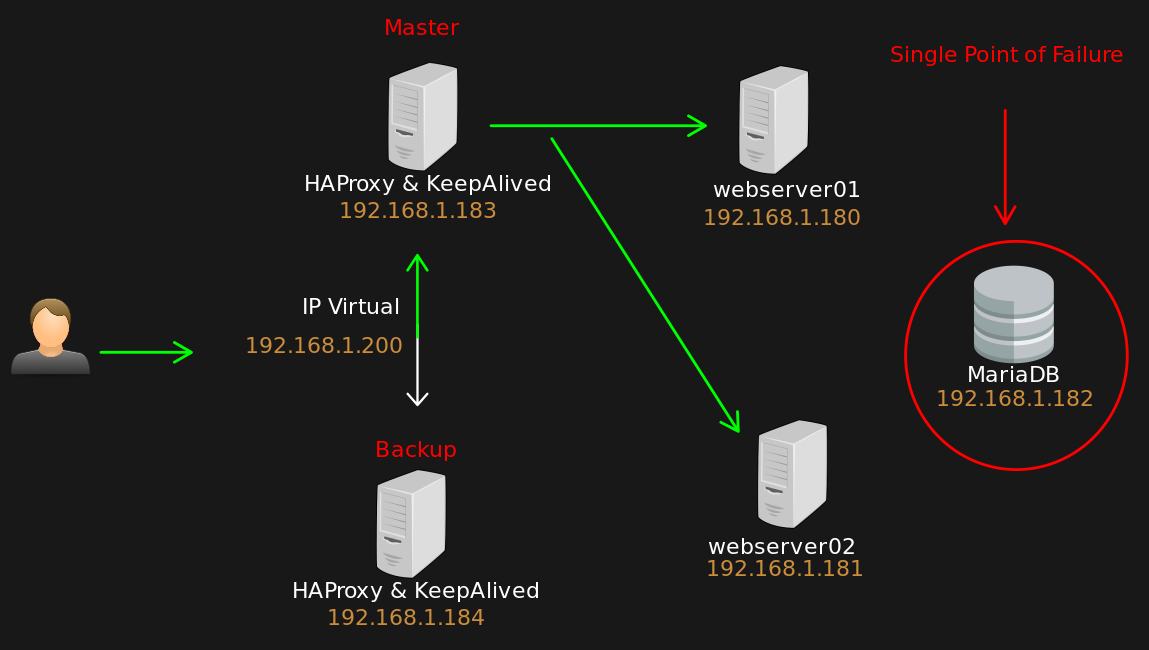
\includegraphics[width=12cm]{imagens/experiencias/02_spof.png}
\caption{Single Point of Failure - Experiência 02}
\label{fig.nav}
\end{figure}


\chapter{Guião}\label{Guião}
\paragraph{}
Em baixo estão descritos os passos para que seja possível criar todo o código da aplicação \emph{web} assim como a base de dados de modo a conseguir-se replicar as experiências que foram mostradas anteriormente.

\section{HAProxy e KeepAlived}
\paragraph{}
Para instalar o HAProxy, bastou fazer \emph{sudo apt install haproxy} em ambos os servidores de HAProxy.\\
Depois foi feita a configuração do ficheiro do HAProxy (\emph{/etc/haproxy/haproxy.cfg}) como descrito na secção de \textbf{Configuração do HAProxy}.
\paragraph{}
Para instalar o KeepAlived, bastou fazer \emph{sudo apt install keepalived} em ambos os servidores de HAProxy.\\
A sua configuração está tambem descrita na secção \textbf{Configuração do Keepalived}.

\section{Aplicação Web}
\subsection{Estrutura da aplicação}

\begin{figure}[H]
\center
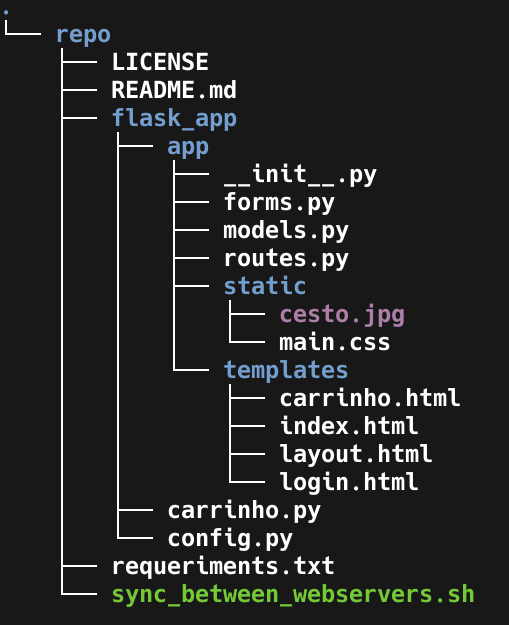
\includegraphics[width=6cm]{imagens/guiao/estrutura_web.png}
\caption{Estrutura da aplicação web - Guião}
\label{fig.nav}
\end{figure}

\clearpage

\subsection{Variáveis de ambiente usadas}

\begin{figure}[H]
\center
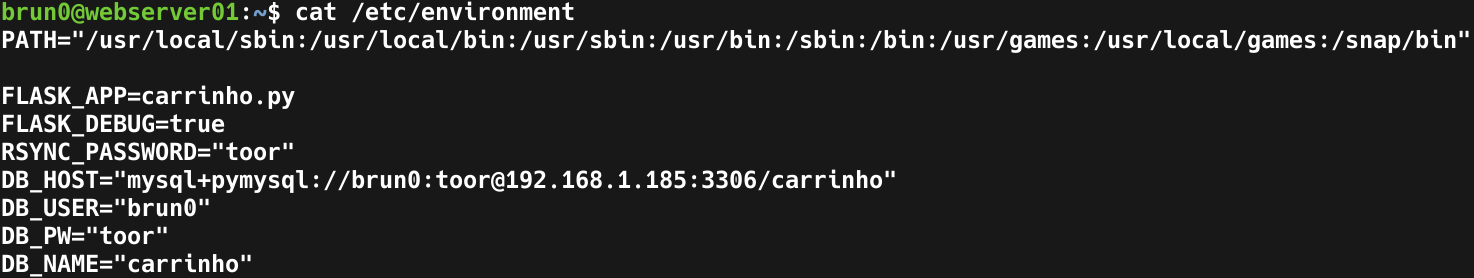
\includegraphics[width=15cm]{imagens/guiao/variaveis_ambiente.png}
\caption{Variáveis de ambiente - Guião}
\label{fig.nav}
\end{figure}



\subsection{requirements.txt}
Para esta aplicação Web são precisas algumas dependências, dependências estas descritas no ficheiro \emph{requeriments.txt}. A maneira mais simples de instalar todas as dependências é criar um ficheiro chamado \emph{requeriments.txt} e depois executar o comando \emph{pip3 install -r requirements.txt}

\begin{lstlisting}
email-validator==1.1.3
entrypoints==0.3
Flask==1.1.1
Flask-Login==0.5.0
Flask-SQLAlchemy==2.5.1
Flask-WTF==0.15.1
httplib2==0.14.0
importlib-metadata==1.5.0
incremental==16.10.1
Jinja2==2.10.1
mariadb==1.0.8
MarkupSafe==1.1.0
more-itertools==4.2.0
oauthlib==3.1.0
pexpect==4.6.0
pyasn1==0.4.2
pyasn1-modules==0.2.1
PyGObject==3.36.0
PyHamcrest==1.9.0
pyinotify==0.9.6
PyJWT==1.7.1
pymacaroons==0.13.0
PyMySQL==1.0.2
PyNaCl==1.3.0
pyOpenSSL==19.0.0
pyrsistent==0.15.5
pyserial==3.4
python-apt==2.0.0+ubuntu0.20.4.6
python-debian===0.1.36ubuntu1
PyYAML==5.3.1
requests==2.22.0
requests-unixsocket==0.2.0
SecretStorage==2.3.1
simplejson==3.16.0
SQLAlchemy==1.4.26
ssh-import-id==5.10
systemd-python==234
Twisted==18.9.0
ufw==0.36
urllib3==1.25.8
wadllib==1.3.3
Werkzeug==0.16.1
WTForms==2.3.3
\end{lstlisting}


\subsection{sync\_between\_webservers.sh}
Este script foi útil para que quando fosse feito um \emph{commit} no \emph{github}, o \emph{webserver01} sincronizasse o código atualizado com o \emph{webserver02}
\begin{lstlisting}
#!/usr/bin/env bash

# automating git stuff

echo "Whats the commit message?"
read message
git add .
git commit -m "${message}"
echo "Pushing data ... "
git push


echo "Syncing to webserver02 ..."
# sync a folder from webserver01 to webserver02
rsync  -rt /home/brun0/repo/ brun0@192.168.1.181:/home/brun0/repo --delete-after
\end{lstlisting}


\subsection{flask\_app}

\subsubsection{carrinho.py}
\begin{lstlisting}
from app import app
\end{lstlisting}


\subsubsection{config.py}
Criar variável de ambiente com o nome \textbf{DB\_HOST}
\begin{lstlisting}
DB_HOST=mysql+pymysql://<username>:<password>@<db_ip>:<db_port>/<db_name>
\end{lstlisting}

\begin{lstlisting}
import os

basedir = os.path.abspath(os.path.dirname(__file__))

class Config(object):
	SECRET_KEY = "something"
	SQLALCHEMY_DATABASE_URI = os.environ.get('DB_HOST')
	SQLALCHEMY_TRACK_MODIFICATIONS = False

\end{lstlisting}

\subsection{app}
\subsubsection{\_\_init\_\_.py}
\begin{lstlisting}
from flask import Flask
from config import Config
from flask_sqlalchemy import SQLAlchemy
from flask_login import LoginManager


app = Flask(__name__)
app.config.from_object(Config)
db = SQLAlchemy(app)

login = LoginManager(app)
login.login_view = "login"

from app import routes,models
\end{lstlisting}


\subsubsection{forms.py}
\begin{lstlisting}
from flask_wtf import FlaskForm
from wtforms import StringField, PasswordField, SubmitField, BooleanField, IntegerField
from wtforms.validators import DataRequired, Length, Email, EqualTo


class LoginForm(FlaskForm):
    email = StringField('Email',validators=[DataRequired(), Email()])
    password = PasswordField('Password', validators=[DataRequired()])
    submit = SubmitField('Login')

class ProductForm(FlaskForm):
        product_type = StringField("Tipo", validators=[DataRequired()])
        quantity = IntegerField("Quantidade", validators=[DataRequired()])
        local = StringField("Local de Compra", validators=[DataRequired()])
        submit = SubmitField('Inserir')
\end{lstlisting}


\subsubsection{models.py}
\begin{lstlisting}
from app import db, login
from werkzeug.security import generate_password_hash, check_password_hash
from flask_login import UserMixin

@login.user_loader
def load_user(id):
    return Clientes.query.get(int(id))

class Clientes(UserMixin, db.Model):
        id_cliente = db.Column(db.Integer, primary_key=True)
        nome = db.Column(db.String(64), index=True, unique=True)
        email = db.Column(db.String(120), index=True, unique=True)
        password = db.Column(db.String(128))
        compras = db.relationship("Compras", backref="cliente")

        def __repr__(self):
                return f"{self.nome}"

        def set_password(self, password):
                self.password = generate_password_hash(password)

        def check_password(self, password):
                return check_password_hash(self.password,password)

        def get_id(self):
                return self.id_cliente

class Compras(db.Model):
        id_compras = (db.Column(db.Integer, primary_key=True))
        tipo = db.Column(db.String(140))
        quantidade = db.Column(db.Integer)
        local = db.Column(db.String(140))
        id_cliente =  db.Column(db.Integer, db.ForeignKey("clientes.id_cliente"))

        def __repr__(self):
                return f"{self.id_compras}"
\end{lstlisting}


\subsubsection{routes.py}
\begin{lstlisting}
from flask import render_template, flash, redirect, url_for, request, jsonify, make_response
from app import app,db
from app.forms import LoginForm, ProductForm
from flask_login import current_user, login_user, logout_user, login_required
from app.models import Clientes, Compras


# index
@app.route("/")
def index():
    return render_template("index.html")

# login
@app.route('/login', methods=['GET', 'POST'])
def login():
        if current_user.is_authenticated:
                return redirect(url_for("carrinho"))

        form = LoginForm()
        if form.validate_on_submit():
                # query a bd
                user = Clientes.query.filter_by(email=form.email.data).first()
                # verifica o resultado da query, se nao existir ...
                if user is None or not user.check_password(form.password.data):
                        flash("Login invalido","danger")
                        return redirect(url_for("login"))
                # se existir faz login
                else:
                        login_user(user)
                return redirect(url_for("carrinho"))
        return render_template("login.html", title="Login", form=form)

# logout
@app.route("/logout")
def logout():
        logout_user()
        flash("Logout com sucesso", "info")
        return redirect(url_for("index"))


# carrinho
@app.route("/carrinho/", methods=["GET", "POST"])
@login_required
def carrinho():
        # lista produtos atuais do cliente
        customer_list = db.session.query(Compras.id_compras.label("id_compras"),
                                        Compras.tipo.label("Tipo"),
                                        Compras.quantidade.label("Quantidade"),
                                        Compras.local.label("Local"))\
                                        .join(Clientes, Compras.id_cliente == Clientes.id_cliente)\
                                        .filter(Compras.id_cliente==current_user.get_id()).all()

    # adicionar produtos ao carrinho
        form = ProductForm()
        if form.validate_on_submit():
                compras = Compras(tipo = form.product_type.data,
                                quantidade = form.quantity.data,
                                local = form.local.data,
                                id_cliente = current_user.get_id())
                db.session.add(compras)
                db.session.commit()

                return redirect(url_for("carrinho"))

        return render_template("carrinho.html", title="Lista", form=form, customer_list=customer_list)

# apagar artigo
@app.route("/apagar_artigo",methods=["POST"])
@login_required
def delete_item():
        # recebe o POST feito no js
        req = request.get_json()
        # aplica a query
        Compras.query.filter_by(id_compras=int(req["id"])).delete()
        db.session.commit()

        return redirect(url_for("carrinho"))
\end{lstlisting}



\subsection{static}
\subsubsection{main.css}
\begin{lstlisting}
  body {
  background: #fafafa;
  color: #333333;
  margin-top: 5rem;
}

h1, h2, h3, h4, h5, h6 {
  color: #444444;
}

.bg-steel {
  background-color: #5f788a;
}

.site-header .navbar-nav .nav-link {
  color: #cbd5db;
}

.site-header .navbar-nav .nav-link:hover {
  color: #ffffff;
}

.site-header .navbar-nav .nav-link.active {
  font-weight: 500;
}

.content-section {
  background: #ffffff;
  padding: 10px 20px;
  border: 1px solid #dddddd;
  border-radius: 3px;
  margin-bottom: 20px;
}

.article-title {
  color: #444444;
}

a.article-title:hover {
  color: #428bca;
  text-decoration: none;
}

.article-content {
  white-space: pre-line;
}

.article-img {
  height: 65px;
  width: 65px;
  margin-right: 16px;
}

.article-metadata {
  padding-bottom: 1px;
  margin-bottom: 4px;
  border-bottom: 1px solid #e3e3e3
}

.article-metadata a:hover {
  color: #333;
  text-decoration: none;
}

.article-svg {
  width: 25px;
  height: 25px;
  vertical-align: middle;
}
\end{lstlisting}


\subsection{templates}
\subsubsection{layout.html}
\begin{lstlisting}
<!DOCTYPE html>
<html>
<head>
    <!-- Required meta tags -->
    <meta charset="utf-8">
    <meta name="viewport" content="width=device-width, initial-scale=1, shrink-to-fit=no">
    <link href="https://use.fontawesome.com/releases/v5.6.3/css/all.css" rel="stylesheet">
    <!-- Bootstrap CSS -->
    <link rel="stylesheet" href="https://maxcdn.bootstrapcdn.com/bootstrap/4.0.0/css/bootstrap.min.css" integrity="sha384-Gn5384xqQ1aoWXA+058RXPxPg6fy4IWvTNh0E263XmFcJlSAwiGgFAW/dAiS6JXm" crossorigin="anonymous">

    <link rel="stylesheet" type="text/css" href="{{ url_for('static', filename='main.css') }}">
    <title>Lista de compras 01</title>
</head>
<body>
    <header class="site-header">
      <nav class="navbar navbar-expand-md navbar-dark bg-steel fixed-top">
        <div class="container">
          <a class="navbar-brand mr-4" href="/">Lista de Compras</a>
          <button class="navbar-toggler" type="button" data-toggle="collapse" data-target="#navbarToggle" aria-controls="navbarToggle" aria-expanded="false" aria-label="Toggle navigation">
            <span class="navbar-toggler-icon"></span>
          </button>
          <div class="collapse navbar-collapse" id="navbarToggle">
            <div class="navbar-nav mr-auto">
            </div>
            <!-- Navbar Right Side -->
            <div class="navbar-nav">
              
              <a class="nav-item nav-link" href="{{ url_for('login') }}">Login</a>
              
              <a class="nav-item nav-link" href="{{ url_for('logout') }}">Logout</a>
              <a class="nav-item nav-link" href="{{ url_for('carrinho') }}">Carrinho</a>
              
            </div>
          </div>
        </div>
      </nav>
    </header>
    <main role="main" class="container">
      <div class="row">

          
            
              
                <div class="alert alert-{{ category }}" style="margin:auto">
                  {{ message }}
                </div>
              
            
        

        
      </div>
    </main>


    <!-- Optional JavaScript -->
    <!-- jQuery first, then Popper.js, then Bootstrap JS -->
    <script src="https://code.jquery.com/jquery-3.1.1.min.js" integrity="sha384-KJ3o2DKtIkvYIK3UENzmM7KCkRr/rE9/Qpg6aAZGJwFDMVNA/GpGFF93hXpG5KkN" crossorigin="anonymous"></script>
    <script src="https://cdnjs.cloudflare.com/ajax/libs/popper.js/1.12.9/umd/popper.min.js" integrity="sha384-ApNbgh9B+Y1QKtv3Rn7W3mgPxhU9K/ScQsAP7hUibX39j7fakFPskvXusvfa0b4Q" crossorigin="anonymous"></script>
    <script src="https://maxcdn.bootstrapcdn.com/bootstrap/4.0.0/js/bootstrap.min.js" integrity="sha384-JZR6Spejh4U02d8jOt6vLEHfe/JQGiRRSQQxSfFWpi1MquVdAyjUar5+76PVCmYl" crossorigin="anonymous"></script>
</body>
</html>
\end{lstlisting}


\subsubsection{index.html}
\begin{lstlisting}



<div class="container ">
<div class="d-flex justify-content-center p-5">
  <img class="mt-5" src="static/cesto.jpg" alt="icon" style="width:350px">
  </div>
  <div class="d-flex justify-content-center text-center p-5">
    <h1>A sua lista de compras<h1/>
    </div>
</div>

\end{lstlisting}


\subsubsection{carrinho.html}
\begin{lstlisting}



<script>
  function remove_entry(){
      var entry = {id:event.srcElement.id};

      fetch(`${window.origin}/apagar_artigo`,{
          method: "POST",
          credentials: "include",
          body: JSON.stringify(entry),
          cache: "no-cache",
          headers: new Headers({
              "content-type":"application/json"
          })
      })

  }
</script>


<div class="col-8">
<div class="container">
      <table class="table table-bordered text-center" id="mytable">
        <thead>
          <tr>
            <th scope="col">ID</th>
            <th scope="col">Tipo</th>
            <th scope="col">Quantidade</th>
            <th scope="col">Local de Compra</th>
            
          </tr>
        </thead>
        <tbody>
          <tr>
            <th scope="row">{{ loop.index }}</th>
            <td>{{ item[1] }}</td>
            <td>{{ item[2] }}</td>
            <td>{{ item[3] }}</td>
            <td>
              <form>
                  <button id={{ item[0] }} type="submit" class="btn btn-danger" onclick="remove_entry();">Apagar</button>
                </form>
            </td>
            
            </tr>
        </tbody>
      </table>
</div>
</div>


<div class="d-flex justify-content-center">
<div class=" d-flex alert alert-dark text-center" style="max-height:62px">Neste momento nao tem nenhum produto no seu cesto
</div>
</div>



  <div class="col-4">
    <div class="content-section">
        <form method="POST" action="">
            {{ form.hidden_tag() }}
            <fieldset class="form-group">
                <legend class="border-bottom mb-4">Carrinho</legend>
                <div class="form-group">
                    {{ form.product_type.label(class="form-control-label") }}
                    
                        {{ form.product_type(class="form-control form-control-lg is-invalid") }}
                        <div class="invalid-feedback">
                            
                                <span>{{ error }}</span>
                            
                        </div>
                    
                        {{ form.product_type(class="form-control form-control-lg") }}
                    
                </div>
                <div class="form-group">
                    {{ form.quantity.label(class="form-control-label") }}
                    
                        {{ form.quantity(class="form-control form-control-lg is-invalid") }}
                        <div class="invalid-feedback">
                            
                                <span>{{ error }}</span>
                            
                        </div>
                    
                        {{ form.quantity(class="form-control form-control-lg") }}
                    
                </div>
                <div class="form-group">
                    {{ form.local.label(class="form-control-label") }}
                    
                        {{ form.local(class="form-control form-control-lg is-invalid") }}
                        <div class="invalid-feedback">
                            
                                <span>{{ error }}</span>
                            
                        </div>
                    
                        {{ form.local(class="form-control form-control-lg") }}
                    
                </div>
            </fieldset>
            <div class="form-group">
              {{ form.submit(class="btn btn-outline-info") }}
            </div>
        </form>
    </div>
    </div>


\end{lstlisting}


\subsubsection{login.html}
\begin{lstlisting}


  <div class="container">
    <div class="content-section">
        <form method="POST" action="">
            {{ form.hidden_tag() }}
            <fieldset class="form-group">
                <legend class="border-bottom mb-4">Log In</legend>
                <div class="form-group">
                    {{ form.email.label(class="form-control-label") }}
                    
                        {{ form.email(class="form-control form-control-lg is-invalid") }}
                        <div class="invalid-feedback">
                            
                                <span>{{ error }}</span>
                            
                        </div>
                    
                        {{ form.email(class="form-control form-control-lg") }}
                    
                </div>
                <div class="form-group">
                    {{ form.password.label(class="form-control-label") }}
                    
                        {{ form.password(class="form-control form-control-lg is-invalid") }}
                        <div class="invalid-feedback">
                            
                                <span>{{ error }}</span>
                            
                        </div>
                    
                        {{ form.password(class="form-control form-control-lg") }}
                    
                </div>
            </fieldset>
            <div class="form-group">
              {{ form.submit(class="btn btn-outline-info") }}
            </div>
        </form>
    </div>


\end{lstlisting}

\section{Base de Dados}
\subsection{Criação da base de dados}
Como a conexão é feita a partir de dois servidores remotos(\textbf{haproxy01} e \textbf{haproxy02}), foi preciso garantir todos os privilegios a esses dois servidores
\begin{lstlisting}
mysql -u root -p
mysql> GRANT ALL ON *.* to <username>@'<ip_haproxy01>' IDENTIFIED BY '<password>';
mysql> GRANT ALL ON *.* to <username>@'<ip_haproxy02>' IDENTIFIED BY '<password>';
mysql> FLUSH PRIVILEGES;
mysql> exit;
sudo service mariadb restart
mysql -u root -p
mysql> create database carrinho;
\end{lstlisting}


\subsection{Criação das tabelas}
\begin{lstlisting}
create table clientes(
    id_cliente int auto_increment,
    nome varchar(255) not null,
    email varchar(255) not null,
    password varchar(255) not null,
    primary key(id_cliente)
);


create table compras(
    id_compras int auto_increment,
    id_cliente int,
    tipo varchar(255) not null,
    quantidade int not null,
    local varchar(255) not null,
    primary key(id_compras),
    foreign key(id_cliente)
    references clientes(id_cliente)
);

\end{lstlisting}

\subsection{Inserção de dados nas tabelas}
\begin{lstlisting}
insert into clientes(nome, email,password) values ("Bruno", "a2019100036@isec.pt", "passwordsegura");
insert into clientes(nome, email,password) values ("Teixeira", "brunoalexandre3@hotmail.com", "passwordsegura");

insert into compras(id_cliente,tipo,quantidade,local) values (1, "Laranjas", 5,"PingoDoce");
insert into compras(id_cliente,tipo,quantidade,local) values (2, "Macas", 2,"PingoDoce");
insert into compras(id_cliente,tipo,quantidade,local) values (1, "Peras", 3,"PingoDoce");
\end{lstlisting}

\begin{acronym}
\acro{isec}[ISEC]{Instituto Superior de Engenharia de Coimbra}
\acro{deis}[DEIS]{Departamento de Engenharia Informática e de Sistemas}
\acro{lei}[LEI]{Licenciatura em Engenharia Informática}
\end{acronym}

\subsection{Selecionar todos os artigos do carrinho do Cliente 1}
\begin{lstlisting}
select compras.id_compras "Id Compras", compras.id_cliente "Id Cliente", clientes.nome "Nome Cliente", compras.tipo, compras.quantidade, compras.local from compras inner join clientes on compras.id_cliente = clientes.id_cliente and clientes.id_cliente = 1;
\end{lstlisting}

\end{document}
